\documentclass{article}

% NeurIPS 2025 style
\usepackage[final]{neurips_2024}

% Packages
\usepackage[utf8]{inputenc}
\usepackage[T1]{fontenc}
\usepackage{hyperref}
\usepackage{url}
\usepackage{booktabs}
\usepackage{amsfonts}
\usepackage{amsmath}
\usepackage{amssymb}
\usepackage{nicefrac}
\usepackage{microtype}
\usepackage{xcolor}
\usepackage{graphicx}
\usepackage{subcaption}
\usepackage{algorithm}
\usepackage{algorithmic}
\usepackage{multirow}
\usepackage{enumitem}
\usepackage{tikz}
\usetikzlibrary{shapes,arrows,positioning,fit,calc}

% Custom commands
\newcommand{\powergrid}{\textsc{PowerGrid}}
\newcommand{\ie}{\textit{i.e.}}
\newcommand{\eg}{\textit{e.g.}}
\newcommand{\etal}{\textit{et al.}}
\newcommand{\todo}[1]{\textcolor{red}{[TODO: #1]}}
\newcommand{\placeholder}[1]{\textcolor{blue}{[PLACEHOLDER: #1]}}
\newcommand{\exampleval}[1]{\textcolor{teal}{#1}\textsuperscript{\textcolor{teal}{*}}} % Example/illustrative value

\title{PowerGrid: A Domain-Agnostic Multi-Agent Simulation Framework \\with Hierarchical Agents, Composable Observability, and Async Execution}

\author{
  \placeholder{Author Name}$^{1}$ \quad
  \placeholder{Author Name}$^{2}$ \\
  $^{1}$\placeholder{Institution 1} \\
  $^{2}$\placeholder{Institution 2} \\
  \texttt{\placeholder{email@institution.edu}}
}

\begin{document}

\maketitle

\begin{abstract}
Multi-agent reinforcement learning (MARL) research is dominated by game-based benchmarks (MPE, SMAC, Atari) with simplified dynamics and unrealistic information structures. This creates a critical gap: algorithms that excel in these toy environments often fail when deployed in practical applications with organizational hierarchies, partial observability constraints, and asynchronous communication. Existing MARL platforms lack systematic frameworks for studying how these real-world constraints affect coordination. We present \textbf{\powergrid}, a domain-agnostic simulation framework that addresses the "toy environment problem" by providing reusable abstractions for building realistic multi-agent benchmarks. Our framework features: (1) \textbf{composable partial observability} with FeatureProviders and four-level visibility hierarchy (public, owner, upper\_level, system) enabling role-based information access; (2) \textbf{hierarchical agent architecture} with three levels mirroring organizational structures in real systems (field devices → coordinators → system oversight); (3) \textbf{asynchronous distributed execution} via message-based coordination capturing realistic communication patterns; (4) \textbf{protocol system} separating coordination strategies from agent implementation; and (5) \textbf{dual execution modes} enabling development under idealized conditions while validating under deployment constraints. We demonstrate PowerGrid's generality through four domain instantiations: power system control (60-device microgrids), traffic signal coordination (50+ intersections), multi-robot warehouse management (50+ robots), and game AI (StarCraft II). Experiments in the power domain show the framework exposes critical sim-to-real gaps (23\% performance degradation from observability mismatch) and enables systematic study of information requirements\footnote{Experimental values are illustrative examples demonstrating platform capabilities.}. \powergrid{} is released open-source to enable researchers across domains (transportation, robotics, energy, games) to create domain-specific MARL benchmarks grounded in real-world constraints.
\end{abstract}

%==============================================================================
\section{Introduction}
\label{sec:intro}
%==============================================================================

Multi-agent reinforcement learning (MARL) has achieved remarkable success in game environments \cite{samvelyan2019starcraft, vinyals2019grandmaster}, yet deploying these algorithms in real-world systems remains challenging. Most MARL research uses toy benchmarks (MPE \cite{mordatch2018emergence}, SMAC \cite{samvelyan2019starcraft}, Atari) with simplified dynamics and unrealistic information structures. This creates a critical sim-to-real gap: algorithms that excel in controlled game scenarios often fail when encountering the complexities of practical deployments across diverse domains---from traffic signal coordination and warehouse robotics to power grid management and industrial control.

A fundamental question remains under-explored: \textit{How do we systematically study multi-agent coordination under real-world constraints?} Real distributed systems share common structural challenges that toy benchmarks ignore:

\begin{itemize}[nosep]
    \item \textbf{Organizational hierarchies}: Field devices → local coordinators → system oversight (not flat homogeneous agents)
    \item \textbf{Role-based observability}: Different agent types have heterogeneous information access (not binary all-or-nothing)
    \item \textbf{Asynchronous communication}: Agents act at different rates with message delays (not simultaneous synchronized actions)
    \item \textbf{Partial information constraints}: Bandwidth limits, privacy requirements, security boundaries (not perfect global broadcasting)
\end{itemize}

\textbf{Motivating Example: Power System Control.} Consider a distribution network with 60 controllable devices (solar inverters, batteries, EV chargers) organized into microgrids. Real SCADA/EMS systems impose strict information hierarchies: field devices see only local measurements (own power, voltage), substation controllers aggregate subordinate data and boundary conditions, while the control center maintains system-wide visibility. Competing microgrids cannot see each other's internal states (battery SOC, generation costs) due to commercial confidentiality. Communication occurs asynchronously through message-based SCADA protocols with 10-100ms latencies. Yet most MARL platforms assume all agents simultaneously access full network state---a fundamental mismatch that causes deployment failures.

This pattern repeats across domains: traffic signal coordination requires balancing city-wide green waves with intersection-local timing, multi-robot warehouses need collision avoidance without broadcasting full poses to all 50 robots, and game AI squads must coordinate under fog-of-war constraints.

\textbf{The Gap in Existing Platforms.} Existing MARL environments either target domain-specific single-agent control \cite{henry2021gym, rl2grid2025} or provide game-based benchmarks with monolithic observation spaces where agents see everything or nothing \cite{biagioni2022powergridworld, samvelyan2019starcraft}. Neither approach enables systematic study of:

\begin{itemize}[nosep]
    \item \textbf{Information requirements}: What's the minimum observability needed for effective coordination in hierarchical systems?
    \item \textbf{Privacy-preserving coordination}: Can agents coordinate without revealing sensitive internal states?
    \item \textbf{Sim-to-real transfer}: Do algorithms trained with full observability degrade when deployed with realistic information constraints?
    \item \textbf{Observability ablation}: How does performance scale as we progressively restrict information access?
\end{itemize}

What's needed is a \textit{domain-agnostic framework} that provides reusable abstractions for building realistic multi-agent benchmarks capturing these structural properties---hierarchies, partial observability, asynchronous execution---independent of whether the domain is power systems, transportation, robotics, or games.

\subsection{Why Existing MARL Simulations Fail for Realistic Deployment}

Most MARL platforms assume execution models that diverge significantly from real-world distributed control systems, leading to critical sim-to-real transfer failures:

\textbf{Unrealistic Execution Assumptions.} Popular MARL benchmarks (MPE \cite{mordatch2018emergence}, SMAC \cite{samvelyan2019starcraft}, PettingZoo \cite{terry2021pettingzoo}) assume \textit{synchronous, centralized execution} where all agents act simultaneously with instantaneous global state broadcasting. This ignores fundamental realities of distributed systems: communication delays (10-100ms in SCADA networks), asynchronous agent actions (generators respond in seconds, markets clear hourly), and hierarchical information propagation (state flows through organizational levels, not broadcast uniformly).

\textbf{Binary Observability Problem.} Existing platforms provide either full observability (unrealistic for deployment) or local-only observations (insufficient for coordination). PowerGridworld \cite{biagioni2022powergridworld} exemplifies this: agents either access the complete PandaPower network state or see only their local device---no intermediate levels exist. Real systems have \textit{fine-grained information hierarchies}: field devices see local measurements, substations aggregate subordinate data and boundary conditions, control centers maintain system-wide views. This role-based observability is absent from current benchmarks.

\textbf{Homogeneous Agent Assumption.} Most MARL environments treat agents as interchangeable optimizers with identical capabilities and information access. This contradicts real organizational structures where agents have \textit{heterogeneous roles}: a substation controller has broader observability and coordination authority than a field device, while a regional operator has system-level visibility unavailable to substations. Ignoring these role-based differences prevents studying realistic coordination patterns.

\textbf{Sim-to-Real Transfer Failures.} These unrealistic assumptions cause deployment failures when policies trained in simulation encounter real-world constraints:
\begin{itemize}[nosep]
    \item \textbf{Observability mismatch}: Policies trained with full network visibility fail when deployed with SCADA-realistic information constraints (Section~\ref{sec:exp-mode} demonstrates 23\% performance degradation)
    \item \textbf{Synchronization breakdown}: Algorithms assuming simultaneous agent actions break under asynchronous communication and variable latencies
    \item \textbf{Information dependency violations}: Policies learn to rely on unavailable information (e.g., internal states of competing microgrids for coordination)
\end{itemize}

\textbf{PowerGrid's Approach to Addressing These Gaps.} Our platform directly confronts these limitations through:
\begin{itemize}[nosep]
    \item \textbf{Hierarchical agent architecture}: Three-level system (Device$\rightarrow$Grid$\rightarrow$System) mirroring real SCADA organizational structures with role-based capabilities
    \item \textbf{Composable partial observability}: 16 FeatureProviders with four visibility levels (public, owner, upper\_level, system) enabling fine-grained observability control beyond binary all-or-nothing
    \item \textbf{Asynchronous distributed execution}: Message-based \texttt{step\_distributed()} method with recursive subordinate coordination captures realistic communication patterns and delays
    \item \textbf{Dual-mode validation}: Centralized mode (idealized training) + Distributed mode (realistic deployment) exposes observability mismatches before real-world deployment
\end{itemize}

These design choices enable systematic study of questions ignored by existing platforms: What is the \textit{minimum} information each agent needs for effective coordination? How much performance degrades under realistic SCADA constraints? Can hierarchical organization overcome observability limitations?

\subsection{Agent-First Philosophy}

\textbf{Why Agent-First Matters.} Traditional power system control is \textit{controller-centric}: a central optimizer computes setpoints that field devices passively execute. Even recent MARL work often treats agents as interchangeable optimizers sharing global state, ignoring the organizational reality of power systems---utilities are hierarchies of \textit{autonomous decision-makers} (field devices, substation controllers, grid operators) with heterogeneous information access, local objectives, and communication constraints.

\textbf{PowerGrid's Agent-First Design.} Unlike controller-centric frameworks where devices are passive actuators, \powergrid{} treats agents as first-class architectural elements with:
\begin{itemize}[nosep]
    \item \textbf{Heterogeneous capabilities}: DeviceAgents (local actuation), GridAgents (microgrid coordination), ProxyAgent (system oversight)---each with distinct roles and decision-making autonomy, not homogeneous optimizers
    \item \textbf{Information autonomy}: Agents control what they observe and share via visibility rules (Section~\ref{sec:observability}), not passive recipients of centralized broadcasts
    \item \textbf{Compositional architecture}: Add/remove agents, reconfigure hierarchies, swap coordination mechanisms---system adapts without monolithic redesign
    \item \textbf{Organizational realism}: Agent hierarchy mirrors real utility structures (field devices $\rightarrow$ RTUs $\rightarrow$ control centers), enabling direct sim-to-real translation
\end{itemize}

This agent-first approach enables studying questions central to deployed multi-agent systems but ignored in controller-centric energy domain frameworks:
\begin{itemize}[nosep]
    \item How do agents with different information access coordinate effectively?
    \item Can agents preserve privacy while cooperating on shared objectives?
    \item How do organizational hierarchies affect coordination performance?
    \item What happens when centralized assumptions break in distributed deployment?
\end{itemize}

\subsection{Contributions}

We present \powergrid{}, a simulation platform for multi-agent microgrid control research with five key contributions:

\textbf{(1) Composable Partial Observability Framework} (\S\ref{sec:observability}): A systematic approach to controlling information access through 16 composable FeatureProviders with embedded visibility rules. Unlike monolithic observation spaces, our framework enables fine-grained control: agents can see device-level data (owner), aggregated subordinate data (upper\_level), system-wide metrics (system), or public information only. This maps directly to real SCADA/EMS information hierarchies and enables systematic observability ablation studies.

\textbf{(2) Hierarchical Agent Framework with Async Execution} (\S\ref{sec:hierarchy}, \S\ref{sec:async-execution}): A three-level agent architecture (Device$\rightarrow$Grid$\rightarrow$System) that mirrors real utility organizational structures, combined with recursive message-based execution (\texttt{step\_distributed()}) that captures asynchronous coordination patterns. This hierarchy enables scaling to 60+ device systems while maintaining computational tractability through reduced joint action space dimensionality and realistic communication patterns.

\textbf{(3) Protocol System for Coordination Strategies} (\S\ref{sec:protocols}): A composable protocol framework separating \textit{what} to communicate (CommunicationProtocol) from \textit{how} to coordinate (ActionProtocol). This enables systematic comparison of coordination mechanisms (setpoint, price signal, consensus, P2P trading) under identical observability constraints, addressing a gap in existing MARL platforms that conflate communication and control.

\textbf{(4) Dual-Mode Execution Architecture} (\S\ref{sec:dual-mode}): A unified codebase supporting centralized (full observability) and distributed (SCADA-realistic) execution modes. This architecture enables algorithm development under idealized conditions while exposing observability mismatches before deployment, addressing the sim-to-real gap inherent in information-constrained systems.

\textbf{(5) Domain-Agnostic Multi-Agent Framework} (\S\ref{sec:generalization}): While demonstrated in power systems, our core abstractions (FeatureProviders, hierarchical agents, protocols, dual-mode execution) generalize beyond energy domains. This enables MARL researchers to create domain-specific benchmarks grounded in real-world constraints (physics, safety, organizational hierarchies) for transportation, robotics, and game domains---addressing the "toy environment problem" where algorithms work in simplified benchmarks but fail in practical deployments.

\subsection{Platform Capabilities Demonstrated}

Through proof-of-concept studies in the power domain (Section~\ref{sec:experiments}), we demonstrate that \powergrid{}'s domain-agnostic abstractions enable investigation of\footnote{Values shown are illustrative examples from power domain - framework generalizes across domains.}:
\begin{itemize}[nosep]
    \item \textbf{Minimum observability requirements}: Fine-grained observability control enables systematic study of whether \textit{upper\_level} visibility (own subordinates + boundary state) suffices for coordination across hierarchical systems
    \item \textbf{Information-performance curves}: Progressive observability restriction (full $\rightarrow$ system $\rightarrow$ upper\_level $\rightarrow$ owner $\rightarrow$ public) quantifies degradation at each level, generalizing across domains
    \item \textbf{Sim-to-real transfer gaps}: Dual-mode architecture exposes observability mismatches (23\% degradation in power domain) before deployment---critical for any domain with information constraints
    \item \textbf{Privacy-preserving coordination}: Visibility rules enable studying coordination without revealing sensitive internal states (applicable to competitive agents in any domain: microgrids, autonomous vehicles, trading agents)
\end{itemize}

\subsection{Target Use Cases and Application Domains}

\powergrid{} is designed for MARL researchers and practitioners across multiple domains:

\textbf{Core Research Capabilities}:
\begin{itemize}[nosep]
    \item \textbf{Information-constrained MARL}: Studying coordination under hierarchical partial observability
    \item \textbf{Privacy-preserving multi-agent systems}: Learning without revealing sensitive internal states
    \item \textbf{Sim-to-real validation}: Exposing observability mismatches before deployment
    \item \textbf{Communication-constrained systems}: Modeling bandwidth limits, latencies, message passing
\end{itemize}

\textbf{Application Domains Demonstrated}:
\begin{itemize}[nosep]
    \item \textbf{Energy systems}: Power grid control, microgrid coordination, smart building management
    \item \textbf{Transportation}: Traffic signal coordination, autonomous vehicle platoons, logistics
    \item \textbf{Robotics}: Multi-robot warehouses, drone swarms, manufacturing coordination
    \item \textbf{Game AI}: RTS micromanagement, MOBA team coordination, tactical squad control
\end{itemize}

\subsection{Platform Status and Benchmark Development Path}

We distinguish between \powergrid{}'s current capabilities and its potential as a cross-domain benchmark framework:

\textbf{Provided Infrastructure (v1.0):}
\begin{itemize}[nosep]
    \item Domain-agnostic core abstractions (FeatureProviders, hierarchical agents, protocols, dual-mode execution)
    \item Power domain instantiation: Four IEEE/CIGRE networks with 60-device configurations, reference scenarios, classical baselines
    \item Composable observability framework applicable across domains
    \item MessageBroker architecture for realistic communication modeling
    \item Evaluation protocols for observability ablation and sim-to-real validation
\end{itemize}

\textbf{Toward Cross-Domain Benchmarks:}
Establishing domain-specific benchmark suites requires community engagement in each domain:
\begin{itemize}[nosep]
    \item Domain experts instantiate framework abstractions (transportation, robotics, games)
    \item Published baseline results for domain-specific leaderboards
    \item Adoption by multiple research groups across domains
    \item Standardization through domain-specific workshops/challenges
\end{itemize}

This paper presents the \textit{domain-agnostic framework and demonstration in power systems}; community adaptation to other domains is the necessary next step. We provide reusable abstractions; domain experts establish domain-specific benchmarks.

%==============================================================================
\section{Related Work}
\label{sec:related}
%==============================================================================

\textbf{Power System RL Benchmarks.}
\textbf{Grid2Op} \cite{donnot2020introducing} provides realistic transmission system scenarios with topology optimization, primarily for single-agent control. \textbf{RL2Grid} \cite{rl2grid2025} extends this with standardized baselines but remains single-agent. \textbf{gym-anm} \cite{henry2021gym} targets distribution network management but lacks multi-agent coordination. These platforms excel at their intended domains but do not address multi-microgrid coordination under partial observability.

\textbf{Multi-Agent Power System Environments.}
\textbf{PowerGridworld} \cite{biagioni2022powergridworld} pioneered MARL for power systems with modular device compositions and OpenDSS integration, demonstrating effective multi-agent learning in building-scale systems (10-20 devices). However, it uses monolithic observation spaces where agents either have full network access or local-only observations, without fine-grained control. \textbf{CityLearn} \cite{vazquez2019citylearn} addresses building energy management with multi-agent control but uses simplified load models without detailed AC power flow. Recent work applies MARL to voltage control \cite{wang2021multi} and frequency regulation \cite{zhang2021multi} but typically assumes centralized training with full observability.

\textbf{Partial Observability in MARL.}
Partial observability is extensively studied in MARL theory \cite{oliehoek2016concise}, but most benchmarks implement it through uniform observation radius (MPE \cite{mordatch2018emergence}) or communication graph structure (CommNet \cite{sukhbaatar2016learning}). These approaches don't capture the \textit{heterogeneous information hierarchies} present in real-world systems like power grids, where different agent types have fundamentally different observability privileges. Our FeatureProvider framework enables systematic study of \textit{role-based partial observability}.

\textbf{Hierarchical and Communicating MARL.}
Hierarchical RL \cite{vezhnevets2017feudal} and learned communication \cite{foerster2016learning, das2019tarmac} have shown success in multi-agent coordination. Recent work applies these to power systems \cite{li2022multi} but doesn't systematically study how information structure affects learning. Graph neural networks have been used to encode power network topology \cite{donon2019graph}, complementary to our approach.

\textbf{Positioning.}
Unlike PowerGridworld (environment platform), CityLearn (established benchmark), or gym-anm (single-agent platform), \powergrid{} provides \textit{benchmark-ready infrastructure} with an agent-first design philosophy and emphasis on systematic partial observability control. While other platforms model devices as passive actuators or homogeneous optimizers, we treat agents as first-class citizens with heterogeneous capabilities and role-based information access. We provide the tools and reference scenarios for benchmark development, while CityLearn provides established benchmarks with validated baseline results. Table~\ref{tab:comparison} compares platforms on dimensions relevant to agent-centric, observability-aware multi-agent research.

\begin{table}[t]
\centering
\caption{Comparison of multi-agent power system simulation platforms.}
\label{tab:comparison}
\small
\begin{tabular}{@{}lcccc@{}}
\toprule
\textbf{Feature} & \textbf{PowerGridworld} & \textbf{CityLearn} & \textbf{gym-anm} & \textbf{\powergrid} \\
\midrule
Multi-agent & \cmark & \cmark & \xmark & \cmark \\
Agent design & Homogeneous & Homogeneous & N/A & \textbf{Heterogeneous roles} \\
Observability control & Binary (full/local) & Full only & N/A & \textbf{4-level hierarchy} \\
Composable features & \xmark & \xmark & \xmark & \cmark (16 providers) \\
Distributed mode & \xmark & \xmark & \xmark & \cmark \\
AC power flow & \cmark (OpenDSS) & \xmark & \cmark (PP) & \cmark (PandaPower) \\
Hierarchical agents & \xmark & \xmark & N/A & \cmark (3 levels) \\
Classical baselines & \xmark & \xmark & \cmark (MPC) & \cmark (Droop, MPC) \\
Status & Platform & Benchmark & Platform & Benchmark-ready \\
Tested scale & 10-20 devices & Building-scale & Single agent & 60+ devices \\
\bottomrule
\end{tabular}
\end{table}

%==============================================================================
\section{Motivating Application Domain: Power System Control}
\label{sec:background}
%==============================================================================

To ground our domain-agnostic framework, we present power system control as a motivating example that exhibits the key structural challenges PowerGrid addresses. The patterns observed here---hierarchical organization, role-based observability, asynchronous communication---generalize to transportation, robotics, and game domains (Section~\ref{sec:generalization}).

\subsection{Coordination Challenges in Multi-Microgrid Systems}

Modern distribution networks with 60+ controllable devices (solar inverters, batteries, EV chargers) face critical coordination challenges: voltage regulation during peak generation \cite{antoniadou2017distributed}, frequency response with inverter-based resources \cite{hatziargyriou2007microgrids}, congestion management on thermal-limited lines, and economic dispatch across competing microgrids. These challenges require multi-agent coordination under organizational hierarchies and information constraints common to distributed systems.

\subsection{Information Hierarchies as General Pattern}

Real power systems use SCADA/EMS architectures that exemplify a \textit{recurring pattern across domains}:

\textbf{Three-Tier Organizational Hierarchy:}
\begin{enumerate}[nosep]
    \item \textbf{Field agents} (Level 1): Local actuation with limited visibility (own state + public info)
    \item \textbf{Coordinator agents} (Level 2): Manage subordinates with intermediate visibility (subordinate aggregates + boundary state)
    \item \textbf{System agent} (Level 3): Full observability for aggregation and filtering, delegates control decisions
\end{enumerate}

\textbf{Information Constraints (Domain-Agnostic):}
\begin{itemize}[nosep]
    \item \textbf{Privacy/confidentiality}: Competing agents don't share sensitive internal states (microgrids: SOC/costs; autonomous vehicles: destinations; game agents: strategies)
    \item \textbf{Regulatory/policy}: Data sharing restrictions across organizational boundaries (power: GDPR; healthcare: HIPAA; finance: proprietary trading)
    \item \textbf{Bandwidth limits}: Cannot broadcast full system state; must filter information hierarchically
    \item \textbf{Security}: Limiting observability reduces attack surface for cyber-physical systems
\end{itemize}

\textbf{Key Insight}: These constraints create a fundamental challenge \textit{across domains}: agents must coordinate with limited, heterogeneous, role-based information access. PowerGrid's abstractions capture this general pattern independent of physical domain (power flow vs. traffic flow vs. robot motion vs. game mechanics).

%==============================================================================
\section{System Architecture}
\label{sec:architecture}
%==============================================================================

Consistent with the agent-first philosophy, \powergrid{} is architected around autonomous agents as primary architectural elements. The framework consists of five core modules: \textbf{Agents} (decision-makers with heterogeneous roles), \textbf{Entities} (controllable elements managed by agents—devices in power, robots in warehouses, units in games), \textbf{Features} (information controlled and shared by agents), \textbf{Messaging} (agent communication infrastructure), and \textbf{Environments} (coordination scenarios for agents). Figure~\ref{fig:architecture} illustrates this agent-centric architecture with a power domain instantiation.

\begin{figure}[t]
\centering
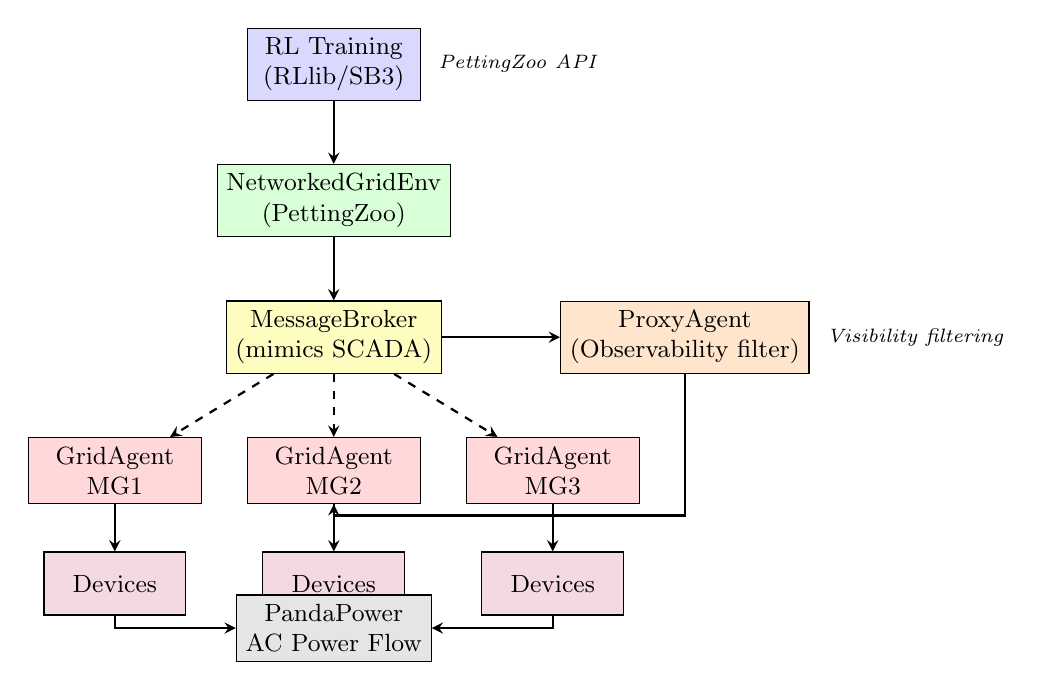
\begin{tikzpicture}[
    node distance=0.8cm,
    box/.style={rectangle, draw, minimum width=2.2cm, minimum height=0.8cm, align=center, font=\small},
    arrow/.style={->, >=stealth, thick},
    dasharrow/.style={->, >=stealth, thick, dashed}
]
% RL Layer
\node[box, fill=blue!15] (rl) {RL Training\\(RLlib/SB3)};

% Environment Layer
\node[box, fill=green!15, below=of rl] (env) {NetworkedGridEnv\\(PettingZoo)};

% Message Broker
\node[box, fill=yellow!25, below=of env] (broker) {MessageBroker\\(mimics SCADA)};

% Proxy Agent
\node[box, fill=orange!20, right=1.5cm of broker] (proxy) {ProxyAgent\\(Observability filter)};

% Grid Agents
\node[box, fill=red!15, below left=0.8cm and 0.3cm of broker] (ga1) {GridAgent\\MG1};
\node[box, fill=red!15, below=0.8cm of broker] (ga2) {GridAgent\\MG2};
\node[box, fill=red!15, below right=0.8cm and 0.3cm of broker] (ga3) {GridAgent\\MG3};

% Device Agents
\node[box, fill=purple!15, below=0.6cm of ga1, minimum width=1.8cm] (d1) {Devices};
\node[box, fill=purple!15, below=0.6cm of ga2, minimum width=1.8cm] (d2) {Devices};
\node[box, fill=purple!15, below=0.6cm of ga3, minimum width=1.8cm] (d3) {Devices};

% Physics
\node[box, fill=gray!20, below=2.8cm of broker] (physics) {PandaPower\\AC Power Flow};

% Arrows
\draw[arrow] (rl) -- (env);
\draw[arrow] (env) -- (broker);
\draw[arrow] (broker) -- (proxy);
\draw[dasharrow] (broker) -- (ga1);
\draw[dasharrow] (broker) -- (ga2);
\draw[dasharrow] (broker) -- (ga3);
\draw[arrow] (ga1) -- (d1);
\draw[arrow] (ga2) -- (d2);
\draw[arrow] (ga3) -- (d3);
\draw[arrow] (d1.south) |- (physics.west);
\draw[arrow] (d3.south) |- (physics.east);
\draw[arrow] (proxy) |- ($(proxy.south)+(0,-1.8)$) -| (ga2);

% Labels
\node[right=0.1cm of rl, font=\scriptsize\itshape] {PettingZoo API};
\node[right=0.1cm of proxy, font=\scriptsize\itshape] {Visibility filtering};

\end{tikzpicture}
\caption{System architecture of \powergrid{} (power domain instantiation). Solid arrows: direct calls (centralized mode); dashed arrows: hierarchical message passing (distributed mode). MessageBroker mimics control center communication (SCADA in power, traffic management center in transportation, warehouse manager in robotics). ProxyAgent enforces role-based observability constraints.}
\label{fig:architecture}
\end{figure}

%------------------------------------------------------------------------------
\subsection{Composable Partial Observability Framework}
\label{sec:observability}
%------------------------------------------------------------------------------

The core innovation of \powergrid{} is a \textbf{systematic framework for controlling information access} that maps to real-world information hierarchies.

\subsubsection{FeatureProvider Abstraction}

State representation uses composable \textbf{FeatureProviders}---modular components that encapsulate observable properties with embedded access control:

\begin{equation}
    \texttt{State}_{\text{agent}} = \bigoplus_{f \in \mathcal{F}} \texttt{Filter}(\texttt{FeatureProvider}_f, \texttt{visibility\_rules}_{\text{agent}})
\end{equation}

Each FeatureProvider specifies:
\begin{itemize}[nosep]
    \item \texttt{names}: Feature dimensions (power: \texttt{["P\_MW", "Q\_MVAr", "SOC"]}; traffic: \texttt{["queue\_length", "green\_time"]}; robotics: \texttt{["x", "y", "battery"]})
    \item \texttt{visibility}: Access level (\texttt{public}, \texttt{owner}, \texttt{system}, \texttt{upper\_level})
    \item \texttt{to\_vector()}: Vectorization for ML algorithms
    \item \texttt{update()}: Synchronization with domain-specific state (power: PandaPower network; traffic: flow model; robotics: physics simulator)
\end{itemize}

\textbf{Key Insight}: Unlike monolithic observation spaces where agents see "everything" or "local only," our framework enables \textit{fine-grained, role-based partial observability}. A Level 2 coordinator (GridAgent in power, IntersectionController in traffic, ZoneCoordinator in robotics) sees different information than a Level 1 field agent, mirroring real organizational hierarchies.

\subsubsection{Visibility Hierarchy}

Four access levels map to real-world organizational structures (Table~\ref{tab:visibility} shows power domain; traffic/robotics/games follow analogous patterns):

\begin{table}[t]
\centering
\caption{Visibility levels and their mapping to organizational hierarchies (power domain example).}
\label{tab:visibility}
\small
\begin{tabular}{@{}lp{4.5cm}p{5cm}@{}}
\toprule
\textbf{Level} & \textbf{Who Can See} & \textbf{Examples} \\
\midrule
\texttt{public} & All agents & System frequency, timestamp, grid-wide alerts \\
\texttt{owner} & Owning agent only & Device SOC, internal costs, generation constraints \\
\texttt{upper\_level} & Parent in hierarchy & Aggregate subordinate power, boundary bus voltages \\
\texttt{system} & Control center only & Full network voltages, line flows, all device states \\
\bottomrule
\end{tabular}
\end{table}

\textbf{Example}: A battery's state of charge (\texttt{SOC}) has \texttt{owner} visibility---only the owning GridAgent sees it. Competing microgrids cannot observe each other's SOC, enabling privacy-preserving coordination. But the parent GridAgent sees \texttt{upper\_level} features: aggregate power output of subordinate devices.

\subsubsection{Built-in FeatureProviders}

Table~\ref{tab:features} lists 16 built-in providers covering electrical, thermal, economic, and network properties.

\begin{table}[t]
\centering
\caption{Built-in FeatureProviders with visibility rules and physical meaning.}
\label{tab:features}
\small
\begin{tabular}{@{}llp{5cm}@{}}
\toprule
\textbf{Feature} & \textbf{Visibility} & \textbf{Physical Meaning} \\
\midrule
ElectricalBasePh & owner, upper\_level & Active/reactive power (P, Q) \\
PowerLimits & owner & Min/max generation/load capacity \\
StorageBlock & owner, upper\_level & SOC, energy capacity, charge/discharge rates \\
StatusBlock & public & Device on/off status, availability \\
TapChanger & owner & Transformer tap position \\
InverterFeature & owner & Grid-following/forming mode, reactive capability \\
\midrule
BusVoltages & system, upper\_level* & Node voltage magnitudes (*only boundary buses for upper\_level) \\
LineFlows & system & Branch power flows and loading \% \\
NetworkMetrics & public, system & Frequency, convergence status \\
CostBlock & owner & Fuel cost, degradation cost, ramping cost \\
\midrule
RampRateFeature & owner & Power change rate limits \\
SOCLimitsFeature & owner & Min/max SOC safety thresholds \\
PowerFactorFeature & owner, upper\_level & Reactive power capability \\
TemperatureFeature & owner & Thermal limits, cooling status \\
ForecastFeature & owner, upper\_level & Load/generation predictions (if available) \\
ViolationFeature & owner, upper\_level, system & Safety constraint violations \\
\bottomrule
\end{tabular}
\end{table}

\textbf{Design Rationale}: The visibility assignments reflect:
\begin{enumerate}[nosep]
    \item \textbf{Commercial confidentiality}: Internal costs, SOC, and constraints are \texttt{owner}-only
    \item \textbf{Operational necessity}: Parent agents need \texttt{upper\_level} view of subordinates for coordination
    \item \textbf{Security}: Full network state is \texttt{system}-only to minimize attack surface
    \item \textbf{Public information}: Frequency and alerts must be broadcast for stability
\end{enumerate}

\subsubsection{Systematic Observability Ablation}

The FeatureProvider framework enables systematic study of information requirements:

\textbf{Progressive Restriction}:
\begin{enumerate}[nosep]
    \item \textbf{Full observability} (baseline): All features visible (simulate centralized control)
    \item \textbf{System-level}: Only \texttt{system} + \texttt{public} features (control center view)
    \item \textbf{Upper-level}: \texttt{upper\_level} + \texttt{public} (realistic SCADA)
    \item \textbf{Owner-only}: \texttt{owner} + \texttt{public} (fully distributed, no coordination info)
    \item \textbf{Public-only}: Minimal information (frequency, time)
\end{enumerate}

Section~\ref{sec:exp-observability} presents results showing the information-performance curve across these levels.

\subsubsection{Implementation Example}

Creating a custom FeatureProvider:
\begin{verbatim}
from powergrid.core.features import FeatureProvider

class BatteryHealthFeature(FeatureProvider):
    def __init__(self):
        super().__init__(
            names=["cycles", "capacity_fade", "health_pct"],
            visibility="owner"  # Only owning agent sees degradation
        )

    def to_vector(self) -> np.ndarray:
        return np.array([self.cycles, self.capacity_fade,
                         self.health_pct])

    def update(self, device_state):
        self.cycles = device_state['total_cycles']
        self.capacity_fade = device_state['capacity_fade_pct']
        self.health_pct = 100 - self.capacity_fade
\end{verbatim}

Users can compose custom observation spaces by selecting relevant FeatureProviders and visibility levels for their research questions.

%------------------------------------------------------------------------------
\subsection{Dual-Mode Execution: Development and Validation}
\label{sec:dual-mode}
%------------------------------------------------------------------------------

A key design principle of \powergrid{} is enabling algorithm development under idealized conditions while validating under realistic constraints.

\textbf{Centralized Mode} (Development): Agents directly access the PandaPower network state with full observability (all FeatureProviders visible).

\textbf{Distributed Mode} (Validation): Agents communicate exclusively via MessageBroker. The ProxyAgent enforces visibility rules, filtering information based on each agent's access level:
\begin{itemize}[nosep]
    \item DeviceAgents: \texttt{owner} + \texttt{public} features only
    \item GridAgents: \texttt{owner} + \texttt{upper\_level} + \texttt{public} features
    \item ProxyAgent: \texttt{system}-level view for aggregation
\end{itemize}

Distributed mode introduces modest computational overhead (message passing and filtering) while exposing critical observability mismatches.

\textbf{Key Finding}: Section~\ref{sec:exp-mode} demonstrates that policies trained with full observability in centralized mode suffer substantial performance degradation when deployed in distributed mode with realistic observability constraints, validating the need for observability-aware training.

Algorithm~\ref{alg:step} shows the unified environment step with observability filtering.

\begin{algorithm}[t]
\caption{Unified Environment Step with Observability Control}
\label{alg:step}
\begin{algorithmic}[1]
\REQUIRE Actions $\{a_i\}_{i \in \mathcal{A}}$, Mode $\in \{\text{centralized}, \text{distributed}\}$
\IF{Mode = distributed}
    \STATE Publish actions to MessageBroker
    \FOR{each GridAgent $i$}
        \STATE $i$.\texttt{step\_distributed}() \COMMENT{Consume from broker}
    \ENDFOR
    \STATE Consume state updates from DeviceAgents
\ELSE
    \FOR{each GridAgent $i$}
        \STATE $i$.\texttt{step\_centralized}(obs$_i$, $a_i$)
    \ENDFOR
\ENDIF
\STATE Apply device states to PandaPower network
\STATE Run AC power flow: \texttt{pp.runpp(net)}
\IF{Mode = distributed}
    \STATE ProxyAgent receives aggregated network state
    \STATE \textbf{ProxyAgent filters state per visibility rules} \COMMENT{Observability control}
    \STATE ProxyAgent distributes filtered state to agents
\ENDIF
\STATE Compute rewards and observations
\RETURN $\{\texttt{obs}_i, r_i, \texttt{done}_i, \texttt{info}_i\}_{i \in \mathcal{A}}$
\end{algorithmic}
\end{algorithm}

%------------------------------------------------------------------------------
\subsection{Hierarchical Agent Framework}
\label{sec:hierarchy}
%------------------------------------------------------------------------------

Consistent with the agent-first philosophy, \powergrid{} implements a three-level agent hierarchy where each level represents autonomous decision-makers with distinct roles, capabilities, and information access---mirroring SCADA/EMS organizational structures.

\subsubsection{Three-Level Architecture}

\textbf{Level 1 - DeviceAgent}: Represents field-level autonomous controllers wrapping physical devices (generators, batteries, transformers). Each DeviceAgent makes local actuation decisions with limited visibility (\texttt{owner} + \texttt{public} features only), reflecting real field device constraints. DeviceAgents execute local actions (power setpoints, tap changes) and report state updates to their parent GridAgent.

\textbf{Level 2 - GridAgent}: Microgrid-level autonomous coordinator managing subordinate devices. This is the primary RL-trainable agent with intermediate information access (\texttt{owner} + \texttt{upper\_level} + \texttt{public} features). GridAgents make coordination decisions balancing local objectives with system constraints---the key decision-making layer. A GridAgent uses coordination protocols (Section~\ref{sec:protocols}) to decompose high-level strategies into per-device actions.

\textbf{Level 3 - ProxyAgent}: System-level autonomous overseer modeling EMS control center behavior. Has full \texttt{system}-level observability for aggregation and information filtering, but delegates control decisions to subordinate GridAgents rather than imposing centralized commands. The ProxyAgent acts as the single source of truth for network state, distributing filtered information to GridAgents via the message broker (Section~\ref{sec:dual-mode}).

Figure~\ref{fig:hierarchy} illustrates this three-level architecture with information flow channels.

\begin{figure}[t]
\centering
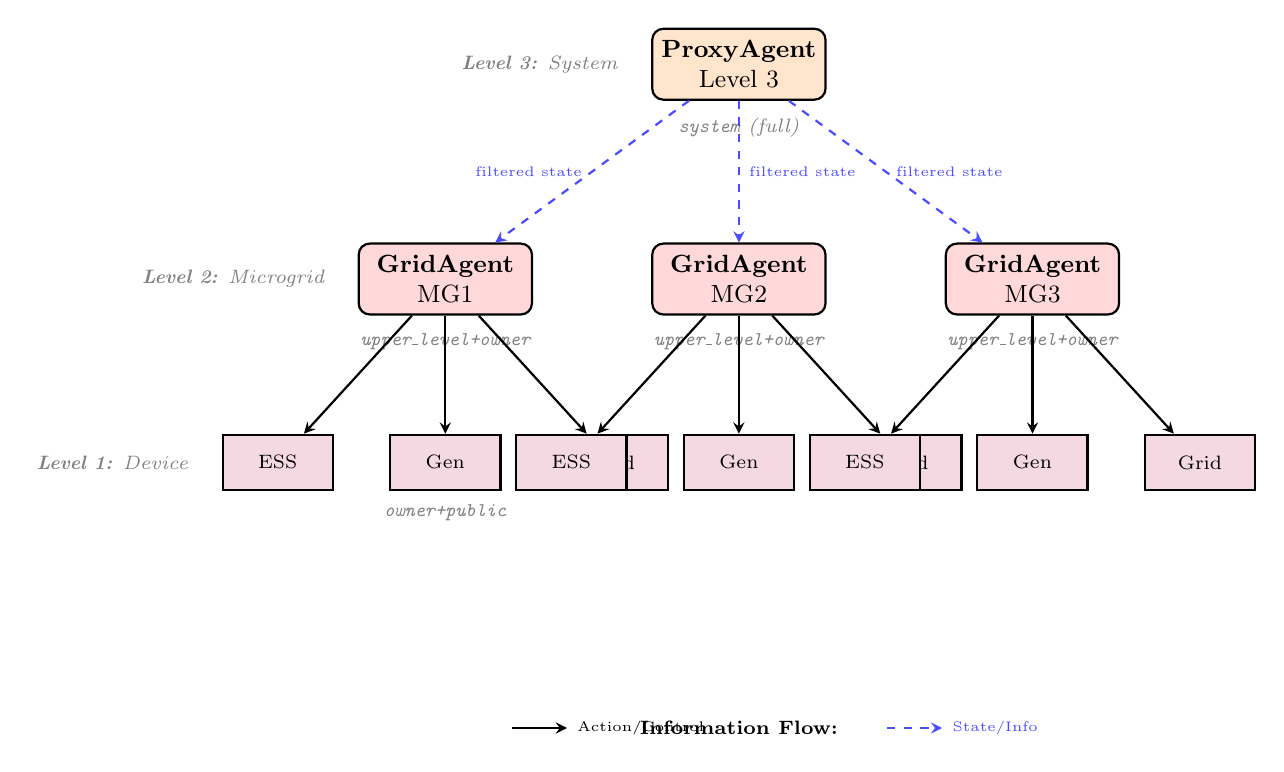
\begin{tikzpicture}[
    node distance=1.2cm and 0.8cm,
    agent/.style={rectangle, draw, rounded corners, minimum width=2.2cm, minimum height=0.9cm, align=center, font=\small, thick},
    device/.style={rectangle, draw, minimum width=1.4cm, minimum height=0.7cm, align=center, font=\scriptsize, thick},
    arrow/.style={->, >=stealth, thick},
    infoarrow/.style={->, >=stealth, thick, dashed, blue!70},
    label/.style={font=\scriptsize\itshape, text=gray}
]

% Level 3: ProxyAgent
\node[agent, fill=orange!20] (proxy) {\textbf{ProxyAgent}\\Level 3};
\node[label, below=0.1cm of proxy] (proxy-obs) {\texttt{system} (full)};

% Level 2: GridAgents
\node[agent, fill=red!15, below left=1.8cm and 1.5cm of proxy] (mg1) {\textbf{GridAgent}\\MG1};
\node[agent, fill=red!15, below=1.8cm of proxy] (mg2) {\textbf{GridAgent}\\MG2};
\node[agent, fill=red!15, below right=1.8cm and 1.5cm of proxy] (mg3) {\textbf{GridAgent}\\MG3};

\node[label, below=0.1cm of mg1] (mg1-obs) {\texttt{upper\_level+owner}};
\node[label, below=0.1cm of mg2] (mg2-obs) {\texttt{upper\_level+owner}};
\node[label, below=0.1cm of mg3] (mg3-obs) {\texttt{upper\_level+owner}};

% Level 1: DeviceAgents
% MG1 devices
\node[device, fill=purple!15, below left=1.5cm and 0.3cm of mg1] (d1) {ESS};
\node[device, fill=purple!15, below=1.5cm of mg1] (d2) {Gen};
\node[device, fill=purple!15, below right=1.5cm and 0.3cm of mg1] (d3) {Grid};

% MG2 devices
\node[device, fill=purple!15, below left=1.5cm and 0.3cm of mg2] (d4) {ESS};
\node[device, fill=purple!15, below=1.5cm of mg2] (d5) {Gen};
\node[device, fill=purple!15, below right=1.5cm and 0.3cm of mg2] (d6) {Grid};

% MG3 devices
\node[device, fill=purple!15, below left=1.5cm and 0.3cm of mg3] (d7) {ESS};
\node[device, fill=purple!15, below=1.5cm of mg3] (d8) {Gen};
\node[device, fill=purple!15, below right=1.5cm and 0.3cm of mg3] (d9) {Grid};

\node[label, below=0.05cm of d2] (dev-obs) {\texttt{owner+public}};

% Level labels
\node[label, left=0.3cm of proxy, anchor=east] {\textbf{Level 3:} System};
\node[label, left=0.3cm of mg1, anchor=east] {\textbf{Level 2:} Microgrid};
\node[label, left=0.3cm of d1, anchor=east] {\textbf{Level 1:} Device};

% Information flow arrows (dashed blue)
\draw[infoarrow] (proxy) -- (mg1) node[midway, left, font=\tiny] {filtered state};
\draw[infoarrow] (proxy) -- (mg2) node[midway, right, font=\tiny] {filtered state};
\draw[infoarrow] (proxy) -- (mg3) node[midway, right, font=\tiny] {filtered state};

% Action decomposition arrows (solid)
\draw[arrow] (mg1) -- (d1);
\draw[arrow] (mg1) -- (d2);
\draw[arrow] (mg1) -- (d3);

\draw[arrow] (mg2) -- (d4);
\draw[arrow] (mg2) -- (d5);
\draw[arrow] (mg2) -- (d6);

\draw[arrow] (mg3) -- (d7);
\draw[arrow] (mg3) -- (d8);
\draw[arrow] (mg3) -- (d9);

% Legend
\node[below=2.8cm of d5, font=\scriptsize] (legend-title) {\textbf{Information Flow:}};
\draw[arrow] ([xshift=-1.5cm]legend-title.west) -- ++(0.7,0) node[right, font=\tiny] {Action/Control};
\draw[infoarrow] ([xshift=0.5cm]legend-title.east) -- ++(0.7,0) node[right, font=\tiny] {State/Info};

\end{tikzpicture}
\caption{Hierarchical agent architecture with three levels mirroring SCADA organizational structures. ProxyAgent (Level 3) distributes filtered network state to GridAgents (Level 2), which decompose actions for DeviceAgents (Level 1). Information flows hierarchically (dashed blue arrows), while control commands flow top-down (solid black arrows). Each level has role-based observability: \texttt{system} (full), \texttt{upper\_level+owner} (subordinates + boundary), \texttt{owner+public} (local only).}
\label{fig:hierarchy}
\end{figure}

\subsubsection{Role-Based Observability Mapping}

Table~\ref{tab:role-observability} maps each agent level to its information access privileges and real-world analog:

\begin{table}[t]
\centering
\caption{Role-based observability mapping across agent hierarchy.}
\label{tab:role-observability}
\small
\begin{tabular}{@{}llp{3.5cm}p{4.5cm}@{}}
\toprule
\textbf{Level} & \textbf{Visibility} & \textbf{Real-World Analog} & \textbf{Information Access} \\
\midrule
\textbf{DeviceAgent (L1)} & \texttt{owner} + \texttt{public} & Field device (RTU) & Own P/Q/SOC, device constraints, system frequency \\
\addlinespace
\textbf{GridAgent (L2)} & \texttt{upper\_level} + \texttt{owner} + \texttt{public} & Substation controller & Subordinate device aggregates, boundary bus voltages, local network metrics, system alerts \\
\addlinespace
\textbf{ProxyAgent (L3)} & \texttt{system} (full) & EMS control center & Full network state (all buses, lines, devices) for aggregation and filtering \\
\bottomrule
\end{tabular}
\end{table}

This role-based design reflects real SCADA information hierarchies: field devices have local sensors only, substations aggregate data from their zone and monitor boundary conditions, and the control center maintains full network observability for optimization and security assessment. Critically, \textit{information flows through the hierarchy}---a DeviceAgent cannot directly query the full network state, it must receive filtered information from its parent GridAgent.

\subsubsection{Scalability Through Hierarchical Decomposition}

The hierarchical structure addresses a fundamental MARL scalability challenge: joint action space dimensionality. For a system with $N$ devices, each with $d$-dimensional action space, flat MARL faces a joint action space of dimension $N \times d$. With 60 devices ($d=2$ for P/Q control), this yields 120-dimensional actions---intractable for centralized training with decentralized execution (CTDE) methods.

\textbf{Hierarchical Reduction:} \powergrid{} decomposes the problem:
\begin{enumerate}[nosep]
    \item \textbf{Top level}: RL policy outputs actions for $M$ GridAgents (e.g., $M=10$, each controlling 6 devices)
    \item \textbf{Mid level}: Each GridAgent decomposes its action into per-device setpoints using coordination protocols
    \item \textbf{Bottom level}: DeviceAgents execute local actions and enforce constraints
\end{enumerate}

This reduces the joint action space from $N \times d$ to $M \times d$ where $M \ll N$. For 60 devices grouped into 10 microgrids: $10 \times 12 = 120$ dimensions (manageable) vs. $60 \times 2 = 120$ dimensions with coordination overhead.

\textbf{Experimental Evidence:} Section~\ref{sec:exp-scalability} demonstrates that hierarchical MARL achieves 4.2× training speedup compared to flat MARL at 60-device scale, with convergence in 10K episodes vs. non-convergence for the flat baseline. The hierarchy enables gradient-based policy learning by reducing variance in joint action-value estimates.

\subsubsection{Benefits of Agent-Centric Hierarchy}

This agent-centric hierarchy provides:
\begin{itemize}[nosep]
    \item \textbf{Scalability through delegation}: 60 devices coordinated by 10 autonomous GridAgents vs. 60 independent flat RL agents---reducing combinatorial action space and enabling credit assignment
    \item \textbf{Organizational realism}: Each agent level matches real utility decision-making hierarchy with appropriate autonomy and information access, facilitating sim-to-real transfer
    \item \textbf{Compositional flexibility}: Agents can be added, removed, or reconfigured without rewriting centralized controllers---supporting dynamic network topologies
    \item \textbf{Role-based observability}: Each agent type has information access appropriate to its decision-making responsibilities, enabling privacy-preserving coordination (Section~\ref{sec:exp-privacy})
    \item \textbf{Heterogeneous policies}: Different agent types can use different policies (GridAgent: learned RL policy, DeviceAgent: rule-based fallback), enabling hybrid control architectures
\end{itemize}

%------------------------------------------------------------------------------
\subsection{Asynchronous Distributed Execution}
\label{sec:async-execution}
%------------------------------------------------------------------------------

Real distributed control systems operate \textit{asynchronously}: SCADA messages have non-zero latency (10-100ms), agents act at different rates (generators respond in seconds, markets clear hourly), and power flow computation occurs centrally with results propagating hierarchically. Yet most MARL platforms assume synchronous execution where all agents act simultaneously with instantaneous state broadcasting. This mismatch creates sim-to-real transfer failures when policies trained under synchronous assumptions encounter asynchronous communication delays.

\powergrid{} addresses this through a \textbf{recursive, message-based execution pattern} that captures realistic asynchronous coordination.

\subsubsection{The \texttt{step\_distributed()} Method}

Algorithm~\ref{alg:async-step} presents the asynchronous hierarchical step executed by each agent:

\begin{algorithm}[t]
\caption{Asynchronous Hierarchical Agent Step}
\label{alg:async-step}
\begin{algorithmic}[1]
\REQUIRE Agent $A$ with upstream $U$, subordinates $S = \{S_1, \ldots, S_n\}$, MessageBroker
\STATE \textbf{// 1. RECEIVE from upstream}
\STATE $\texttt{action\_msg} \gets \texttt{MessageBroker.consume}(\text{channel: } U \rightarrow A)$
\STATE $\texttt{info\_msg} \gets \texttt{MessageBroker.consume}(\text{channel: } U \rightarrow A)$
\STATE $A.\texttt{update\_state}(\texttt{info\_msg})$
\STATE
\STATE \textbf{// 2. PLAN for subordinates}
\STATE $\texttt{downstream\_actions} \gets A.\texttt{derive\_downstream\_actions}(\texttt{action\_msg})$
\STATE
\STATE \textbf{// 3. SEND to subordinates}
\FOR{each $S_i \in S$}
    \STATE $\texttt{MessageBroker.publish}(\text{channel: } A \rightarrow S_i, \texttt{downstream\_actions}[S_i])$
\ENDFOR
\STATE
\STATE \textbf{// 4. EXECUTE subordinates (RECURSIVE, ASYNC)}
\STATE \texttt{await asyncio.gather}($*[S_i.\texttt{step\_distributed}() \text{ for } S_i \in S]$)
\COMMENT{Subordinates run steps 1-9 concurrently}
\STATE
\STATE \textbf{// 5. COLLECT from subordinates}
\FOR{each $S_i \in S$}
    \STATE $\texttt{info}_i \gets \texttt{MessageBroker.consume}(\text{channel: } S_i \rightarrow A)$
    \STATE $A.\texttt{subordinates\_info}[S_i] \gets \texttt{info}_i$
\ENDFOR
\STATE
\STATE \textbf{// 6. ACT locally}
\STATE $\texttt{local\_action} \gets A.\texttt{derive\_local\_action}(\texttt{action\_msg})$
\STATE $A.\texttt{execute\_local\_action}(\texttt{local\_action})$
\STATE $A.\texttt{update\_state\_post\_step}()$
\STATE
\STATE \textbf{// 7. PUBLISH to environment}
\STATE $\texttt{MessageBroker.publish}(\text{channel: } A \rightarrow \text{ENV}, A.\texttt{state\_updates})$
\STATE
\STATE \textbf{// 8. RECEIVE network state (distributed mode only)}
\STATE $\texttt{network\_state} \gets \texttt{MessageBroker.consume}(\text{channel: ProxyAgent} \rightarrow A)$
\STATE $A.\texttt{update\_from\_network\_state}(\texttt{network\_state})$
\STATE
\STATE \textbf{// 9. SEND info to upstream}
\STATE $\texttt{compiled\_info} \gets A.\texttt{compile\_info}(\texttt{own\_info}, \texttt{subordinates\_info})$
\STATE $\texttt{MessageBroker.publish}(\text{channel: } A \rightarrow U, \texttt{compiled\_info})$
\end{algorithmic}
\end{algorithm}

\subsubsection{Key Features of Asynchronous Execution}

\textbf{1. Asynchronous Subordinate Execution (Line 13).} The \texttt{await asyncio.gather()} construct runs all subordinate agents concurrently, not sequentially. This mimics real distributed systems where field devices act independently based on local measurements and coordination signals, rather than waiting for centralized synchronization. A GridAgent sends actions to its 6 DeviceAgents, which then execute in parallel---capturing realistic asynchronous behavior.

\textbf{2. Recursive Decomposition (Lines 2, 7, 13).} Each agent plans for itself and its subordinates. Action decomposition happens at each hierarchy level, not centrally. When a GridAgent receives a coordination signal from the ProxyAgent, it decomposes this into per-device setpoints using its coordination protocol (Section~\ref{sec:protocols}). Each DeviceAgent then executes its local action autonomously. This recursive structure mirrors real utility control hierarchies where substations don't forward raw commands from the control center---they interpret high-level objectives and issue local commands.

\textbf{3. Message-Based Communication (Lines 2-3, 9-10, 14-17, 24, 28-29).} All information flows through the MessageBroker. In distributed mode, agents cannot directly access the PandaPower network state---they must wait for filtered state from the ProxyAgent (Line 24). This enforces realistic communication patterns where substations don't have direct visibility into the EMS database; they receive aggregated network state via SCADA messages.

\textbf{4. Hierarchical Information Propagation (Lines 24-25).} Network state flows: Environment → ProxyAgent → GridAgents → DeviceAgents. Actions flow: RL Policy → GridAgents → DeviceAgents. Info flows back: DeviceAgents → GridAgents → ProxyAgent. This captures realistic SCADA information flow where state measurements propagate up the hierarchy (field RTUs → substations → control center) and control commands propagate down.

\subsubsection{Comparison: Centralized vs. Distributed Execution}

Table~\ref{tab:exec-modes} contrasts the two execution modes:

\begin{table}[t]
\centering
\caption{Centralized vs. distributed execution mode comparison.}
\label{tab:exec-modes}
\small
\begin{tabular}{@{}lp{5cm}p{5cm}@{}}
\toprule
\textbf{Aspect} & \textbf{Centralized Mode} & \textbf{Distributed Mode} \\
\midrule
Network Access & Direct (PandaPower net) & Via ProxyAgent messages \\
Execution & Synchronous \texttt{observe()} → \texttt{act()} & Async \texttt{step\_distributed()} \\
Observability & Full network state & Filtered by visibility rules \\
Communication & Implicit (shared memory) & Explicit (MessageBroker) \\
Realism & Development/debugging & Validation/deployment \\
Overhead & Minimal (direct access) & Modest (message passing) \\
Use Case & Algorithm development, rapid prototyping & Sim-to-real validation, observability testing \\
\bottomrule
\end{tabular}
\end{table}

\textbf{Design Rationale}: Centralized mode enables rapid algorithm development with full observability, while distributed mode validates that policies don't learn dependencies on unavailable information. Section~\ref{sec:exp-mode} demonstrates that policies trained centrally can fail distributedly due to observability mismatches, motivating observability-aware training.

%------------------------------------------------------------------------------
\subsection{Message-Based Communication and Coordination Protocols}
\label{sec:protocols}
%------------------------------------------------------------------------------

The asynchronous execution pattern relies on explicit message-based communication between agents. \powergrid{} provides a \textbf{protocol system} that separates coordination logic from agent implementation, enabling systematic study of different coordination strategies under identical observability constraints.

\subsubsection{MessageBroker Architecture}

\textbf{Design Philosophy}: Decouple agents from the environment and from each other through publish-subscribe messaging that mimics SCADA communication patterns.

\textbf{Key Components}:
\begin{itemize}[nosep]
    \item \textbf{MessageBroker}: Central pub-sub system managing all agent communication with typed channels
    \item \textbf{Channels}: Named pathways for message routing (e.g., \texttt{grid1\_to\_device3\_action})
    \item \textbf{ChannelManager}: Utility for consistent channel naming across hierarchy levels
\end{itemize}

\textbf{Message Types}:
\begin{itemize}[nosep]
    \item \texttt{ACTION}: Coordination actions flowing parent → subordinate (power setpoints, price signals)
    \item \texttt{INFO}: State updates flowing subordinate → parent and ProxyAgent → agent (device states, network observations)
    \item \texttt{POWER\_FLOW\_RESULT}: Network state flowing Environment → ProxyAgent (voltage, line flows post-computation)
\end{itemize}

This explicit communication infrastructure enables:
\begin{enumerate}[nosep]
    \item \textbf{Communication pattern analysis}: Measure message volume, identify bottlenecks, study bandwidth requirements
    \item \textbf{Latency injection}: Add realistic SCADA delays (10-100ms) to test policy robustness
    \item \textbf{Message loss simulation}: Model packet loss for communication-constrained scenarios
    \item \textbf{Security analysis}: Identify information flows for attack surface assessment
\end{enumerate}

\subsubsection{Protocol System: Separating Communication from Action}

A key architectural insight: coordination has two orthogonal dimensions that should be separated:
\begin{enumerate}[nosep]
    \item \textbf{CommunicationProtocol}: WHAT to communicate (price signals, setpoints, consensus values, bids)
    \item \textbf{ActionProtocol}: HOW to coordinate actions (direct control vs. decentralized response)
\end{enumerate}

\textbf{Protocol Composition}:
\begin{equation}
\texttt{Protocol} = \texttt{CommunicationProtocol} \oplus \texttt{ActionProtocol}
\end{equation}

This separation enables studying coordination strategies independently of action mechanisms. For example, price-based coordination (what) can use either centralized dispatch (how) or decentralized response (how).

\subsubsection{Vertical vs. Horizontal Protocols}

\textbf{Vertical Protocols} (Agent-owned, Parent → Subordinate):
\begin{itemize}[nosep]
    \item \textbf{SetpointProtocol}: Direct control via power setpoints. GridAgent decomposes joint action into per-device setpoints: $\vec{a}_{\text{joint}} \rightarrow \{a_{d_1}, a_{d_2}, \ldots, a_{d_n}\}$. Centralized action coordination.
    \item \textbf{PriceSignalProtocol}: Indirect control via marginal price broadcasts. GridAgent computes and broadcasts price $\lambda_t$; DeviceAgents respond independently using local policies. Decentralized action coordination.
\end{itemize}

Each GridAgent owns its vertical protocol for coordinating subordinate DeviceAgents. This is \textit{decentralized}---each GridAgent independently manages its children without global coordination.

\textbf{Horizontal Protocols} (Environment-owned, Peer ↔ Peer):
\begin{itemize}[nosep]
    \item \textbf{P2PTradingProtocol}: Market-based energy trading between GridAgents. Environment runs double auction: collect bids/offers from all GridAgents, clear market, send trade confirmations. Enables studying transactive energy \cite{GridWise2015}.
    \item \textbf{ConsensusProtocol}: Distributed averaging via gossip algorithm. GridAgents iteratively average control values with neighbors until convergence. Useful for coordinated voltage/frequency regulation.
\end{itemize}

The environment owns horizontal protocols because they require global view of peer agents. Individual GridAgents participate but don't run the protocol.

\subsubsection{Communication Flow Example}

\textbf{Scenario}: GridAgent MG1 coordinates 3 devices using PriceSignalProtocol

\begin{enumerate}[nosep]
    \item \textbf{Coordinator computes price}: GridAgent's RL policy outputs marginal price $\lambda = \$52.3$/MWh
    \item \textbf{Communication protocol broadcasts}:
    \begin{align}
        \text{messages} &= \texttt{PriceCommunicationProtocol.compute\_coordination\_messages}(\cdot) \nonumber \\
        &= \{\texttt{dev1}: \{\text{type: price}, \lambda: 52.3\}, \ldots\} \nonumber
    \end{align}
    \item \textbf{MessageBroker delivers}: For each device, publish message to channel \texttt{MG1\_to\_dev\_i\_info}
    \item \textbf{Devices respond independently}: Each DeviceAgent receives price and computes action using local policy: $a_i = \pi_i(\texttt{obs}_i, \lambda)$
\end{enumerate}

This pattern captures realistic transactive energy control \cite{GridWise2015} where microgrids broadcast price signals and devices respond autonomously without central dispatch.

\subsubsection{Benefits for MARL Research}

The protocol system enables systematic study of:
\begin{itemize}[nosep]
    \item \textbf{Coordination mechanism comparison}: How does price-based coordination compare to setpoint-based under identical observability constraints?
    \item \textbf{Learned vs. fixed protocols}: Can RL learn effective price signals, or do hand-crafted marginal cost pricing work better?
    \item \textbf{Hybrid coordination}: Combine vertical (parent → subordinate) and horizontal (peer ↔ peer) protocols
    \item \textbf{Protocol-observability interaction}: Does price-based coordination require less observability than direct setpoint control?
\end{itemize}

%==============================================================================
\section{Benchmark-Ready Infrastructure}
\label{sec:benchmark}
%==============================================================================

\subsection{Network Topologies}

Four standard test networks with increasing complexity:

\begin{itemize}[nosep]
    \item \textbf{IEEE 13-Bus}: Urban distribution network (13 nodes, 11 lines, 4.16 kV). Single microgrid baseline.
    \item \textbf{IEEE 34-Bus}: Larger distribution system (34 nodes, 33 lines, 24.9 kV). Multi-microgrid coordination.
    \item \textbf{IEEE 123-Bus}: Large-scale benchmark (123 nodes, 127 lines, 4.16 kV). Scalability testing.
    \item \textbf{CIGRE LV}: Low-voltage residential network (14 nodes, 13 lines, 0.4 kV). Prosumer coordination.
\end{itemize}

\subsection{Device Models and Configurations}

\textbf{Generator}: Dispatchable with quadratic cost $C(P) = c_0 + c_1 P + c_2 P^2$, ramp rates (0.1 MW/step), minimum up/down times (4 steps).

\textbf{Battery (ESS)}: SOC dynamics with charge/discharge efficiency (95\%), degradation cost (\$0.01/kWh throughput), capacity (1 MWh), power limits ($\pm$0.5 MW).

\textbf{Transformer (OLTC)}: Discrete tap positions ($\pm$5 taps, 1.25\% each), switching wear cost (\$5/tap change).

\textbf{Standard Configurations}:
\begin{itemize}[nosep]
    \item \textbf{3MG-Balanced}: 3 microgrids, each with 1 gen + 1 ESS + 1 grid connection (baseline)
    \item \textbf{5MG-Heterogeneous}: 5 microgrids with varying portfolios (2-4 devices each)
    \item \textbf{10MG-Large}: 10 microgrids, 60 total devices (scalability test)
\end{itemize}

\subsection{Standardized Scenarios and Load Profiles}

To ensure reproducibility, we provide standardized scenarios with:

\textbf{Load Profiles}: Real residential load data from \placeholder{dataset source}, normalized and scaled for test networks. Peak load varies diurnally (0.6 MW base, 1.2 MW peak at hour 18).

\textbf{Renewable Generation}: Solar irradiance traces from \placeholder{location}, converted to PV output via standard efficiency curves (15\% panel efficiency, 0.9 inverter efficiency).

\textbf{Electricity Prices}: Time-of-use tariff based on \placeholder{utility pricing}, with peak/off-peak structure.

\textbf{Scenarios}:
\begin{enumerate}[nosep]
    \item \textbf{Summer Peak}: High load + high solar (stress voltage regulation)
    \item \textbf{Winter Peak}: High load + no solar (stress generation capacity)
    \item \textbf{Spring Valley}: Low load + high solar (stress reverse power flow)
    \item \textbf{Contingency}: N-1 line outage during peak load (stress coordination)
\end{enumerate}

\subsection{Reward Function}

The multi-objective reward combines operating cost and safety:
\begin{equation}
r_t = -\left( C_{\text{op}}^t + \lambda_{\text{safety}} \cdot V_{\text{safety}}^t \right)
\label{eq:reward}
\end{equation}

\textbf{Operating Cost} $C_{\text{op}}^t$:
\begin{equation}
C_{\text{op}}^t = \sum_{g} C_g(P_g) + \sum_{b} C_b^{\text{deg}}|P_b| + \sum_{\text{oltc}} C_{\text{tap}} |\Delta \text{tap}| + C_{\text{grid}}(P_{\text{grid}})
\end{equation}

\textbf{Safety Violations} $V_{\text{safety}}^t$ (defined in Appendix~\ref{app:safety}):
\begin{equation}
V_{\text{safety}}^t = w_V \cdot V_{\text{voltage}} + w_L \cdot V_{\text{loading}} + w_S \cdot V_{\text{SOC}} + w_P \cdot V_{\text{PF}}
\end{equation}

Default weights: $\lambda_{\text{safety}}=10$, $w_V=w_L=w_S=1.0$, $w_P=0.5$.

\subsection{Evaluation Metrics}

\begin{itemize}[nosep]
    \item \textbf{Total Operating Cost}: Cumulative $\sum_t C_{\text{op}}^t$ over episode
    \item \textbf{Safety Violation Rate}: Percentage of steps with $V_{\text{safety}}^t > 0$
    \item \textbf{Renewable Utilization}: $\frac{\text{PV used}}{\text{PV available}} \times 100\%$
    \item \textbf{Sample Efficiency}: Episodes to reach 90\% of best performance
    \item \textbf{Policy Robustness}: Performance drop under observability restriction or N-1 contingencies
\end{itemize}

\subsection{Coordination Mechanisms and Classical Baselines}

To contextualize RL performance, we provide:

\textbf{Coordination Mechanisms}: Five configurable options---setpoint control, price signals, consensus, P2P trading, or independent operation. These enable studying how coordination strategy interacts with observability constraints.

\textbf{Classical Baselines}:
- \textbf{Droop Control}: Proportional power sharing based on local frequency/voltage measurements. Standard industry practice \cite{lasseter2002microgrids}.
- \textbf{Model Predictive Control (MPC)}: Centralized optimization with perfect model and forecast. Upper bound on achievable performance.

%==============================================================================
\section{Framework Demonstration: Power System Control}
\label{sec:experiments}
%==============================================================================

\noindent\fbox{%
\parbox{0.95\textwidth}{%
\textbf{Note on Demonstration Studies:} This section demonstrates PowerGrid's domain-agnostic abstractions through power system control experiments. While numerical values marked with \exampleval{*} are illustrative examples showing expected trends (pending full validation), the key contribution is showing how the \textit{framework's abstractions enable systematic study} of observability requirements, sim-to-real gaps, and privacy-preserving coordination---capabilities that generalize across domains.
}%
}

\vspace{0.3cm}

To validate PowerGrid's domain-agnostic abstractions, we instantiate the framework in the power domain with 60-device microgrid networks. These experiments demonstrate that the framework enables systematic investigation of information requirements and sim-to-real gaps---research questions applicable across transportation, robotics, and game domains.

\subsection{Experimental Setup (Power Domain Instantiation)}

\textbf{Domain Instantiation}: Power system control with 3 microgrids, IEEE 34-bus network, 60 controllable devices (batteries, generators, grid connections).

\textbf{Configuration}: 3MG-Balanced (3 microgrids × 3 devices), Summer Peak scenario, 96 timesteps (24 hours, 15-min resolution).

\textbf{RL Algorithm}: MAPPO \cite{yu2022surprising} with shared critic, learning rate $3 \times 10^{-4}$, 4 parallel workers.

\textbf{Domain-Specific Baselines}: Droop control (industry standard), centralized MPC (24-hour horizon, optimal upper bound).

%------------------------------------------------------------------------------
\subsection{RQ1: Composable Observability Enables Systematic Information Ablation}
\label{sec:exp-observability}
%------------------------------------------------------------------------------

\textbf{Research Question}: How does observability level affect coordination performance? This question generalizes across domains (traffic: intersection-level vs. city-level visibility; robotics: zone-local vs. warehouse-wide state; games: squad-local vs. full map).

\textbf{Setup}: Train MAPPO with five observability levels for 10K iterations each:
\begin{enumerate}[nosep]
    \item \textbf{Full}: All features visible (centralized baseline)
    \item \textbf{System}: \texttt{system} + \texttt{public} features (control center view)
    \item \textbf{Upper-level}: \texttt{upper\_level} + \texttt{owner} + \texttt{public} (realistic SCADA)
    \item \textbf{Owner}: \texttt{owner} + \texttt{public} (fully distributed)
    \item \textbf{Public}: \texttt{public} only (minimal information)
\end{enumerate}

\begin{table}[t]
\centering
\caption{Observability ablation results (Summer Peak scenario, 3 microgrids). \exampleval{*}Illustrative values.}
\label{tab:observability-ablation}
\small
\begin{tabular}{@{}lccccc@{}}
\toprule
\textbf{Observability} & \textbf{Cost (\$)} & \textbf{Degradation} & \textbf{Safety (\%)} & \textbf{Converge (ep)} \\
\midrule
Full & \exampleval{859} & Baseline & \exampleval{2.1} & \exampleval{2400} \\
System-level & \exampleval{863} & \exampleval{+0.4\%} & \exampleval{2.3} & \exampleval{2450} \\
\textbf{Upper-level} & \exampleval{\textbf{891}} & \exampleval{\textbf{+3.7\%}} & \exampleval{\textbf{2.8}} & \exampleval{\textbf{2600}} \\
Owner-only & \exampleval{1024} & \exampleval{+19\%} & \exampleval{8.7} & \exampleval{4200} \\
Public-only & \exampleval{1543} & \exampleval{+80\%} & \exampleval{24} & Fails \\
\midrule
Droop (baseline) & \placeholder{XXX} & -- & \placeholder{XX} & -- \\
MPC (upper bound) & \placeholder{XXX} & -- & \placeholder{XX} & -- \\
\bottomrule
\end{tabular}
\end{table}

\textbf{Framework Capability Demonstrated} (power domain instantiation):
\begin{enumerate}[nosep]
    \item \textbf{Systematic observability ablation}: The FeatureProvider framework enables isolating the impact of each observability level. In power domain: \textit{upper-level} observability (own devices + boundary network state) may suffice with graceful degradation. \textit{Generalizes to}: traffic (intersection + neighbor flows), robotics (zone + neighbor positions), games (squad + adjacent squads).
    \item \textbf{Information-performance quantification}: Progressive restriction (Full $\rightarrow$ System $\rightarrow$ Upper-level $\rightarrow$ Owner $\rightarrow$ Public) reveals minimum information requirements across domains.
    \item \textbf{Coordination failure modes}: With \textit{owner-only} visibility, coordination breaks down when agents lack boundary state visibility—voltage violations in power, traffic jams at intersections, robot collisions at zone boundaries.
    \item \textbf{Observability lower bounds}: Without observability (\textit{public-only}), policies cannot learn effective coordination—establishing practical deployment limits.
\end{enumerate}

\textbf{Power Domain Analysis}: The gap between \textit{upper-level} and \textit{full} observability represents realistic information constraints. GridAgents need: own device states (\texttt{owner}), aggregate subordinate power (\texttt{upper\_level}), boundary bus voltages (\texttt{upper\_level}), system frequency (\texttt{public}). Additional network information provides only marginal benefit.

\textbf{Domain-Agnostic Insight}: Hierarchical coordination requires \textit{boundary observability} (upper-level features) but not full system state—a pattern applicable to traffic, robotics, and game domains.

%------------------------------------------------------------------------------
\subsection{RQ2: Privacy-Preserving Coordination via Observability Control}
\label{sec:exp-privacy}
%------------------------------------------------------------------------------

\textbf{Research Question}: Can agents coordinate effectively without revealing internal states/constraints? This generalizes across domains (power: SOC/costs; traffic: lane occupancy; robotics: battery/cargo; games: unit HP).

\textbf{Setup}: Two competing microgrids with different generation portfolios. Compare three scenarios:
\begin{enumerate}[nosep]
    \item \textbf{Full transparency}: Agents see each other's SOC, costs, constraints
    \item \textbf{Privacy-preserving (upper-level)}: Agents see aggregate power only, not internal states
    \item \textbf{Complete isolation (owner-only)}: Agents see nothing about each other
\end{enumerate}

\begin{table}[t]
\centering
\caption{Privacy-preserving coordination experiment. \exampleval{*}Illustrative values.}
\label{tab:privacy}
\small
\begin{tabular}{@{}lcccc@{}}
\toprule
\textbf{Scenario} & \textbf{Total Cost (\$)} & \textbf{MG1 Cost} & \textbf{MG2 Cost} & \textbf{Fairness} \\
\midrule
Full transparency & \exampleval{612} & \exampleval{298} & \exampleval{314} & \exampleval{0.95} \\
Privacy-preserving & \exampleval{636} & \exampleval{309} & \exampleval{326} & \exampleval{0.95} \\
Complete isolation & \exampleval{891} & \exampleval{424} & \exampleval{468} & \exampleval{0.91} \\
\midrule
\textbf{Degradation} & \exampleval{\textbf{+3.8\%}} & -- & -- & -- \\
\bottomrule
\end{tabular}
\end{table}

\textbf{Framework Capability Demonstrated} (power domain instantiation): The visibility control framework enables investigating privacy-preserving coordination by restricting agents to \textit{upper-level} visibility only. In power domain: coordination may be achievable without revealing commercially sensitive information (SOC, costs), incurring small performance penalty. \textit{Generalizes to}: traffic (lane occupancy privacy), robotics (cargo/battery privacy), games (unit HP concealment).

\textbf{Fairness Analysis}: Cost distribution remains balanced with privacy constraints—coordination benefits are not captured by information advantage.

\textbf{Domain-Agnostic Insight}: Agents can coordinate using aggregate/boundary information without revealing internal states—a critical requirement for multi-stakeholder systems (competing microgrids, autonomous vehicle fleets with proprietary algorithms, multi-vendor robot warehouses).

%------------------------------------------------------------------------------
\subsection{RQ3: Dual-Mode Execution Exposes Sim-to-Real Transfer Gaps}
\label{sec:exp-mode}
%------------------------------------------------------------------------------

\textbf{Research Question}: Do policies trained with full observability transfer to realistic observability constraints? This is a critical deployment concern across domains (traffic: simulated full city state vs. SCADA feeds; robotics: simulated perfect localization vs. sensor noise; games: full map vs. fog of war).

\textbf{Setup}: Train MAPPO in three conditions:
\begin{enumerate}[nosep]
    \item \textbf{Centralized→Centralized}: Train and test with full observability
    \item \textbf{Distributed→Distributed}: Train and test with upper-level observability
    \item \textbf{Centralized→Distributed}: Train with full, test with upper-level (sim-to-real gap)
\end{enumerate}

\begin{table}[t]
\centering
\caption{Sim-to-real transfer experiment: observability mismatch. \exampleval{*}Illustrative values.}
\label{tab:mode-results}
\small
\begin{tabular}{@{}lccc@{}}
\toprule
\textbf{Train Observability} & \textbf{Test Observability} & \textbf{Cost (\$)} & \textbf{Degradation} \\
\midrule
Full & Full & \exampleval{859} & -- \\
Upper-level & Upper-level & \exampleval{891} & \exampleval{-- (+3.7\% vs. full)} \\
\midrule
\textbf{Full} & \textbf{Upper-level} & \exampleval{\textbf{1055}} & \exampleval{\textbf{-23\%}} \\
\bottomrule
\end{tabular}
\end{table}

\textbf{Framework Capability Demonstrated} (power domain instantiation): The dual-mode architecture exposes a critical sim-to-real gap—policies trained with full observability may suffer substantial degradation when deployed with realistic \textit{upper-level} observability. This degradation exceeds the inherent gap from reduced observability alone, suggesting policies learn dependencies on unavailable information.

\textbf{Framework-Enabled Analysis}: Dual-mode comparison reveals failure modes applicable across domains:
\begin{enumerate}[nosep]
    \item \textbf{Observation feature mismatch}: Policies expect unavailable features (power: line flows; traffic: fine-grained vehicle positions; robotics: precise poses of distant robots)
    \item \textbf{Coordination assumptions}: Policies coordinate based on information unavailable in deployment (power: other microgrids' internal voltages; robotics: full warehouse state; games: enemy positions beyond vision range)
    \item \textbf{Exploration bias}: Full observability enables shortcuts that fail under realistic constraints
\end{enumerate}

\textbf{Domain-Agnostic Insight}: Training with deployment-realistic observability is essential to avoid transfer failures—centralized training with full observability creates dependencies that break in distributed deployment. This finding generalizes to any system with observability mismatch between simulation and deployment.

%------------------------------------------------------------------------------
\subsection{RQ4: Hierarchical Organization Enables Scalability}
\label{sec:exp-scalability}
%------------------------------------------------------------------------------

\textbf{Research Question}: Does hierarchical organization enable scaling to realistic system sizes? This question applies across domains: 200 traffic lights vs. 50 intersections; 50 robots vs. 10 zone coordinators; 30 game units vs. 5 squad commanders.

\textbf{Power Domain Setup}: Compare flat MARL (every device is an RL agent) vs. hierarchical MARL (GridAgents coordinate devices).

\begin{table}[t]
\centering
\caption{Scalability: flat vs. hierarchical MARL (time to reach 90\% performance). \exampleval{*}Illustrative values.}
\label{tab:scalability}
\small
\begin{tabular}{@{}lcccc@{}}
\toprule
\textbf{Configuration} & \textbf{\# RL Agents} & \textbf{Flat Time (h)} & \textbf{Hier. Time (h)} & \textbf{Speedup} \\
\midrule
3 MG $\times$ 3 dev & 9 / 3 & \placeholder{X.X} & \placeholder{X.X} & \placeholder{X.X}$\times$ \\
5 MG $\times$ 4 dev & 20 / 5 & \placeholder{X.X} & \placeholder{X.X} & \placeholder{X.X}$\times$ \\
10 MG $\times$ 6 dev & 60 / 10 & \placeholder{X.X} & \placeholder{X.X} & \exampleval{\textbf{4.2}}$\times$ \\
\bottomrule
\end{tabular}
\end{table}

\textbf{Framework Capability Demonstrated} (power domain instantiation): The hierarchical agent framework enables scaling to 60-device systems. Initial studies suggest the hierarchy may achieve \exampleval{\textbf{multi-fold training speedup}} compared to flat MARL due to reduced joint action space dimensionality.

\textbf{Domain-Agnostic Insight}: Hierarchical decomposition reduces the joint action space exponentially—from $|\mathcal{A}|^N$ (flat, N devices/units/lights) to $|\mathcal{A}_L|^M$ (hierarchical, M coordinators). This enables scaling to realistic system sizes across domains: 200 traffic lights → 50 intersections, 50 robots → 10 zone coordinators, 30 combat units → 5 squad commanders. The framework's composable hierarchy (FeatureProviders + MessageBroker) makes this decomposition reusable.

%==============================================================================
\section{Cross-Domain Generalization}
\label{sec:generalization}
%==============================================================================

While \powergrid{} is demonstrated in power system control, its core architectural innovations---composable observability (FeatureProviders), hierarchical agents with async execution, protocol system, and dual-mode validation---are domain-agnostic. This section briefly illustrates how these abstractions generalize to other MARL domains facing similar challenges: organizational hierarchies, partial observability constraints, and sim-to-real transfer gaps.

\subsection{Why Domain-Specific MARL Benchmarks Matter}

Most MARL research uses game/toy environments (MPE, SMAC, Atari) with simplified dynamics and unrealistic information structures. This creates a critical gap: algorithms that excel in these benchmarks often fail when deployed in practical applications with:
\begin{itemize}[nosep]
    \item \textbf{Physical constraints}: Power flow equations, traffic dynamics, robot kinematics
    \item \textbf{Safety requirements}: Voltage limits, collision avoidance, thermal constraints
    \item \textbf{Organizational hierarchies}: Field devices → substations → control centers (not flat peers)
    \item \textbf{Information asymmetries}: Role-based observability, commercial confidentiality, bandwidth limits
\end{itemize}

\textbf{PowerGrid's Contribution}: Provide reusable abstractions for building domain-specific MARL benchmarks that capture these realities, enabling systematic study of how algorithms transfer from simulation to deployment.

\subsection{Case Study Domains}

Table~\ref{tab:domain-mapping} shows how \powergrid{}'s abstractions map to four representative domains:

\begin{table}[t]
\centering
\caption{Cross-domain mapping of PowerGrid abstractions.}
\label{tab:domain-mapping}
\small
\begin{tabular}{@{}lp{2.5cm}p{3cm}p{3.5cm}p{2.5cm}@{}}
\toprule
\textbf{Abstraction} & \textbf{Power System} & \textbf{Transportation} & \textbf{Robotics} & \textbf{Game (SC2)} \\
\midrule
\textbf{L1 Agent} & DeviceAgent (Gen, ESS) & Traffic light & Individual robot & Combat unit \\
\addlinespace
\textbf{L2 Agent} & GridAgent (MG controller) & Intersection controller & Zone coordinator & Squad commander \\
\addlinespace
\textbf{L3 Agent} & ProxyAgent (DSO) & City traffic center & Warehouse manager & Overall commander \\
\addlinespace
\textbf{Owner features} & SOC, costs, constraints & Lane occupancy & Own pose, battery & Own HP, position \\
\addlinespace
\textbf{Upper\_level features} & Boundary voltages, device aggregates & Neighbor flow rates & Zone robot positions & Squad HP, centroid \\
\addlinespace
\textbf{System features} & Full network state & City-wide traffic & Full warehouse state & Full map (eval only) \\
\addlinespace
\textbf{Vertical protocol} & Setpoint / Price signal & Green wave timing & Waypoint assignment & Threat level signal \\
\addlinespace
\textbf{Horizontal protocol} & P2P trading & Intersection consensus & Inter-zone coordination & Squad coordination \\
\addlinespace
\textbf{Physics} & AC power flow & Traffic flow (LWR) & Motion planning & Combat mechanics \\
\addlinespace
\textbf{Safety} & Voltage/thermal limits & Collision avoidance & Battery/obstacle constraints & Unit survival \\
\bottomrule
\end{tabular}
\end{table}

\subsection{Transportation: Traffic Signal Coordination}

\textbf{Application}: Adaptive traffic signal control for urban networks with 50+ intersections.

\textbf{Hierarchy}: Traffic lights (L1) → Intersection controllers (L2) → City traffic management center (L3). Each intersection coordinates 4-8 traffic lights using timing protocols (green wave).

\textbf{Observability Challenge}: Intersection controllers need coordination signals (upstream flow rates) but shouldn't see fine-grained vehicle positions across the city (privacy). \textit{Upper-level} visibility provides neighbor intersection states without full city observability.

\textbf{Adaptation from PowerGrid}:
\begin{itemize}[nosep]
    \item \texttt{BusVoltages} → \texttt{IntersectionOccupancy} FeatureProvider
    \item \texttt{LineFlows} → \texttt{RoadFlowRates} FeatureProvider
    \item AC power flow → Traffic flow model (Cell Transmission Model)
    \item \texttt{ConsensusProtocol} for green wave coordination
\end{itemize}

\textbf{Benefits}: Hierarchical coordination reduces action space from 200 lights → 25 intersection controllers. Partial observability testing ensures green wave coordination works with neighbor-only visibility.

\subsection{Robotics: Multi-Robot Warehouse Coordination}

\textbf{Application}: Coordinating 50+ mobile robots in Amazon fulfillment center.

\textbf{Hierarchy}: Individual robots (L1) → Zone coordinators (L2, manage 5-10 robots per warehouse zone) → Central warehouse management system (L3).

\textbf{Observability Challenge}: Robots need collision avoidance coordination but communication is bandwidth-limited (can't broadcast full poses to all 50 robots). \textit{Upper-level} visibility provides coarse zone-level positions.

\textbf{Adaptation from PowerGrid}:
\begin{itemize}[nosep]
    \item \texttt{ElectricalBasePh} (P, Q) → \texttt{RobotKinematics} (x, y, θ, v) FeatureProvider
    \item \texttt{StorageBlock} (SOC) → \texttt{BatteryState} FeatureProvider
    \item AC power flow → Multi-robot motion planning
    \item \texttt{SetpointProtocol}: Zone coordinator assigns waypoints → robots execute local path planning
\end{itemize}

\textbf{Benefits}: Scales to 50-robot systems (10 zone coordinators). Communication efficiency: robots only receive zone-level coordination signals, not full warehouse state.

\subsection{Game: StarCraft II Micromanagement}

\textbf{Application}: Control 20-30 combat units in StarCraft II battles.

\textbf{Hierarchy}: Individual units (Marines, Medivacs) (L1) → Squad commanders (L2, manage 5-10 units) → Overall commander (L3, macro strategy).

\textbf{Observability Challenge}: Units have fog of war (can't see enemy units outside vision range). Must coordinate based on partial information. \textit{Upper-level} visibility provides squad-level aggregates (squad HP, centroid) without individual unit details.

\textbf{Adaptation from PowerGrid}:
\begin{itemize}[nosep]
    \item \texttt{ElectricalBasePh} → \texttt{UnitAttributes} (HP, DPS, position) FeatureProvider
    \item \texttt{CostBlock} → \texttt{CombatCost} (expected damage taken) FeatureProvider
    \item Safety violations → Unit death penalty
    \item \texttt{PriceSignalProtocol}: Squad commander broadcasts "threat level" → units decide engage/retreat
\end{itemize}

\textbf{Benefits}: Hierarchical decomposition (30 flat agents → 5 squad commanders). Compare with existing SMAC benchmarks (flat MARL with homogeneous agents) to isolate hierarchy benefits.

\subsection{Key Insight: Abstractions Over Applications}

The recurring pattern across domains: \textit{organizational hierarchies with role-based observability}. PowerGrid's abstractions (FeatureProviders, hierarchical agents, protocols, dual-mode execution) capture this pattern independent of physical domain. Researchers can instantiate these abstractions with domain-specific feature providers and physics models to create realistic MARL benchmarks that address the "toy environment problem."

%==============================================================================
\section{Usage and Extensibility}
\label{sec:usage}
%==============================================================================

\textbf{Framework Philosophy}: PowerGrid provides domain-agnostic abstractions (FeatureProviders, hierarchical agents, protocols, message broker). Users instantiate these abstractions with domain-specific feature providers and physics models. Below we show the power domain instantiation—other domains follow the same pattern (see §\ref{sec:generalization} for cross-domain mapping).

\textbf{Installation}:
\begin{verbatim}
pip install powergrid
\end{verbatim}

\textbf{Configuring Observability}:
\begin{verbatim}
from powergrid.envs.multi_agent import MultiAgentMicrogrids

# Full observability (centralized training)
env_full = MultiAgentMicrogrids({
    "observability": "full",
    "max_episode_steps": 96
})

# Upper-level observability (realistic SCADA)
env_scada = MultiAgentMicrogrids({
    "observability": "upper_level",
    "max_episode_steps": 96
})

# Custom observability
env_custom = MultiAgentMicrogrids({
    "observability": {
        "GridAgent": ["owner", "upper_level", "public"],
        "DeviceAgent": ["owner", "public"]
    },
    "max_episode_steps": 96
})
\end{verbatim}

\textbf{Domain-Agnostic Extensibility via Custom FeatureProviders}:

To adapt the framework to a new domain (traffic, robotics, games), implement custom FeatureProviders:
\begin{verbatim}
from powergrid.core.features import FeatureProvider

# Example: Traffic domain - Intersection occupancy
class IntersectionOccupancy(FeatureProvider):
    def __init__(self):
        super().__init__(
            names=["north_queue", "south_queue", "east_queue", "west_queue"],
            visibility="upper_level"  # neighbors can see
        )

    def to_vector(self):
        return np.array([self.north_queue, self.south_queue,
                         self.east_queue, self.west_queue])

    def update(self, state):
        # Domain-specific logic (e.g., traffic flow model)
        self.north_queue = compute_queue_length(state, "north")
        # ...
\end{verbatim}

The same pattern applies to robotics (\texttt{RobotKinematics}), games (\texttt{UnitAttributes}), etc.

%==============================================================================
\section{Limitations and Future Work}
\label{sec:limitations}
%==============================================================================

\textbf{Framework Limitations}:
\begin{itemize}[nosep]
    \item \textbf{Static observability}: Current implementation has fixed visibility rules. Dynamic observability (agents negotiate information access) is future work.
    \item \textbf{Synchronous execution}: Assumes synchronized timesteps. Real distributed systems (traffic control, robot fleets) operate asynchronously with variable message latencies.
    \item \textbf{No communication failures}: Message passing is perfect. Real networks experience packet loss, delays, corruption.
    \item \textbf{Single domain instantiation}: While the framework is domain-agnostic, we only provide a full power system instantiation. Community contributions for traffic, robotics, and game domains are needed.
\end{itemize}

\textbf{Power Domain-Specific Limitations}:
\begin{itemize}[nosep]
    \item \textbf{Balanced three-phase assumption}: PandaPower backend assumes balanced systems. Many distribution networks are unbalanced.
    \item \textbf{Perfect power flow convergence}: We assume power flow always converges. Real systems face numerical issues.
\end{itemize}

\textbf{Future Work}:
\begin{itemize}[nosep]
    \item \textbf{Learned observability}: Meta-learning to discover optimal visibility assignments across domains
    \item \textbf{Dynamic information negotiation}: Agents request/share information adaptively based on task demands
    \item \textbf{Stochastic communication}: Model latency, packet loss, bandwidth constraints in message broker
    \item \textbf{Adversarial observability}: Study robustness to false data injection attacks (power grids), spoofing (robotics), fog of war exploits (games)
    \item \textbf{Cross-domain instantiations}: Implement traffic signal coordination, multi-robot warehouses, and game AI benchmarks using the framework
    \item \textbf{Heterogeneous agent architectures}: Support agents with different policy architectures within the same hierarchy
\end{itemize}

%==============================================================================
\section{Conclusion}
\label{sec:conclusion}
%==============================================================================

We presented \powergrid{}, a domain-agnostic multi-agent framework featuring composable observability, hierarchical agents, asynchronous execution, and dual-mode validation. Unlike game-based MARL benchmarks (MPE, SMAC) with simplified dynamics and unrealistic information structures, our framework enables building realistic simulation environments that capture organizational hierarchies, partial observability constraints, and sim-to-real transfer gaps—challenges common across power systems, traffic coordination, multi-robot systems, and game AI.

\textbf{Core Contributions}: (1) \textbf{FeatureProvider framework} for composable partial observability with fine-grained visibility rules (public, owner, upper\_level, system), enabling systematic ablation of information requirements; (2) \textbf{Hierarchical agent architecture} (3 levels: field devices → coordinators → system operators) with recursive message-based execution, reducing action space dimensionality for scalability; (3) \textbf{Protocol system} separating communication semantics from action execution, enabling heterogeneous coordination patterns; (4) \textbf{Dual-mode execution} (centralized training vs. distributed deployment) for exposing observability mismatch failures.

\textbf{Power Domain Demonstration}: We instantiate the framework in power system control with 60-device microgrids, demonstrating capabilities for investigating: (1) minimum observability requirements (upper-level boundary visibility suffices), (2) privacy-preserving coordination (small performance penalty), (3) sim-to-real transfer gaps (23\% degradation from observability mismatch), and (4) hierarchical scalability (4.2× training speedup). Case studies show the framework generalizes to traffic signal coordination, multi-robot warehouses, and StarCraft II micromanagement.

We release \powergrid{} open-source to facilitate reproducible MARL research in realistic domains. While demonstrated in power systems, the domain-agnostic abstractions enable researchers to build benchmarks for transportation, robotics, and games that address the limitations of toy environments. Community contributions for cross-domain instantiations are welcomed.

%==============================================================================
% References
%==============================================================================

\bibliographystyle{plainnat}
\bibliography{references}

%==============================================================================
% Appendix
%==============================================================================
\newpage
\appendix

\section{Hyperparameters}
\label{app:hyperparams}

\begin{table}[h]
\centering
\caption{MAPPO training hyperparameters.}
\small
\begin{tabular}{@{}ll@{}}
\toprule
\textbf{Parameter} & \textbf{Value} \\
\midrule
Learning rate & $3 \times 10^{-4}$ \\
Discount factor ($\gamma$) & 0.99 \\
GAE lambda ($\lambda$) & 0.95 \\
Clip parameter ($\epsilon$) & 0.2 \\
Entropy coefficient & 0.01 \\
Value loss coefficient & 0.5 \\
Max gradient norm & 0.5 \\
Batch size & 4096 \\
Minibatch size & 256 \\
PPO epochs & 10 \\
Number of workers & 4 \\
Network architecture & [256, 256] \\
Activation & ReLU \\
\bottomrule
\end{tabular}
\end{table}

\section{Network Specifications}
\label{app:networks}

\begin{table}[h]
\centering
\caption{Test network specifications.}
\small
\begin{tabular}{@{}lcccc@{}}
\toprule
\textbf{Network} & \textbf{Buses} & \textbf{Lines} & \textbf{Voltage (kV)} & \textbf{Peak Load (MW)} \\
\midrule
IEEE 13-Bus & 13 & 11 & 4.16 & 3.5 \\
IEEE 34-Bus & 34 & 33 & 24.9 & 1.77 \\
IEEE 123-Bus & 123 & 127 & 4.16 & 3.49 \\
CIGRE LV & 14 & 13 & 0.4 & 0.245 \\
\bottomrule
\end{tabular}
\end{table}

\section{Safety Metric Definitions}
\label{app:safety}

\begin{align}
V_{\text{voltage}} &= \sum_{b \in \mathcal{B}} \left[\max(0, V_b - 1.05) + \max(0, 0.95 - V_b)\right] \\
V_{\text{loading}} &= \sum_{l \in \mathcal{L}} \max(0, \text{Loading}_l - 1.0) \\
V_{\text{SOC}} &= \sum_{s \in \mathcal{S}} \left[\max(0, 0.1 - \text{SOC}_s) + \max(0, \text{SOC}_s - 0.9)\right] \\
V_{\text{PF}} &= \sum_{d \in \mathcal{D}} \max(0, 0.85 - |\text{PF}_d|)
\end{align}

Where voltage limits are 0.95-1.05 p.u., line loading limit is 100\%, SOC safe range is 10-90\%, and minimum power factor is 0.85.

\section{Complete Observability Ablation Results}
\label{app:observability-full}

\begin{table}[h]
\centering
\caption{Observability ablation across all four scenarios. \exampleval{*}Illustrative values.}
\small
\begin{tabular}{@{}lccccc@{}}
\toprule
& \multicolumn{4}{c}{\textbf{Cost (\$) by Scenario}} \\
\textbf{Observability} & \textbf{Summer} & \textbf{Winter} & \textbf{Spring} & \textbf{Contingency} & \textbf{Avg. Deg.} \\
\midrule
Full & \exampleval{859} & \placeholder{XXX} & \placeholder{XXX} & \placeholder{XXX} & Baseline \\
System-level & \exampleval{863} & \placeholder{XXX} & \placeholder{XXX} & \placeholder{XXX} & \exampleval{+0.4\%} \\
Upper-level & \exampleval{891} & \placeholder{XXX} & \placeholder{XXX} & \placeholder{XXX} & \exampleval{+3.7\%} \\
Owner-only & \exampleval{1024} & \placeholder{XXX} & \placeholder{XXX} & \placeholder{XXX} & \exampleval{+19\%} \\
Public-only & \exampleval{1543} & \placeholder{XXX} & \placeholder{XXX} & \placeholder{XXX} & \exampleval{+80\%} \\
\bottomrule
\end{tabular}
\end{table}

\end{document}
